\documentclass[12pt,a4paper]{report}

% ---------- Paket dasar ----------
\usepackage[utf8]{inputenc}
\usepackage[T1]{fontenc}
\usepackage[indonesian]{babel}
\usepackage{lipsum}

% ---------- Paket matematika & gambar ----------
\usepackage{amsmath,amssymb}
\usepackage{graphicx}
\usepackage{caption}
\usepackage{subcaption}
\usepackage{float}
\usepackage{algorithm}
\usepackage{algpseudocode}
\usepackage{listings}
\usepackage{xcolor}

\lstdefinestyle{godestyle}{
    language=Go,
    basicstyle=\ttfamily\small,
    keywordstyle=\color{black},
    commentstyle=\color{black!50!black},
    stringstyle=\color{black!60!black},
    numbers=left,
    numberstyle=\tiny\color{black},
    stepnumber=1,
    numbersep=8pt,
    showstringspaces=false,
    breaklines=true,
    frame=single,
    tabsize=4,
    captionpos=b
}
\usepackage{multicol}
\bibliographystyle{IEEEtran}
% ---------- Paket lain ----------
\usepackage[most]{tcolorbox}
\usepackage{forest}
\usepackage{hyperref}
\usepackage{fancyhdr}

\usepackage{titlesec}

\usepackage{titlesec}
\usepackage{longtable}
\usepackage{array} % untuk menentukan lebar kolom
\usepackage{booktabs} % gaya tabel lebih elegan
\usepackage[table]{xcolor}



% Tambah jarak aman dari header dan footer:	
\setlength{\headheight}{14.5pt}   % wajib cukup besar untuk fancyhdr
\setlength{\headsep}{55pt}      % jarak header ke teks
\setlength{\footskip}{28pt}     % jarak teks ke footer
\usepackage[a4paper,top=3cm,bottom=3cm,left=3cm,right=3cm]{geometry}

% Semua gambar dari folder public dan subfoldernya
\graphicspath{{public/}{public/01-pendahuluan/}{public/02-dasar-teori/}{public/03-implementasi/}}

% --- Pengaturan header & footer ---
\pagestyle{fancy}
\fancyhf{} % clear all

% --- Paksa semua halaman (termasuk awal chapter) memakai fancy ---
\fancypagestyle{plain}{%
	\fancyhf{}%
	\fancyhead[L]{%
		
\includegraphics[height=1.1cm]{logo-itb}\hspace{0.3cm}%
		
\includegraphics[height=1.1cm]{logo-stei}\hspace{0.3cm}%
	}%
	\fancyhead[R]{%
		\begin{minipage}{9cm}
			\raggedleft\bfseries IF2211 Strategi Algoritma\\
			\normalsize Laporan Akhir Tugas Besar 2\\
			Semester II 2025/2026
		\end{minipage}
	}%
	\renewcommand{\headrulewidth}{0.4pt}%
	\fancyfoot[L]{\small v1.0}%
	\fancyfoot[C]{\small Halaman \thepage}%
	\fancyfoot[R]{\small }%
	\renewcommand{\footrulewidth}{0.4pt}%
}


\fancyhead[L]{%
	
\includegraphics[height=1.5cm]{logo-itb}\hspace{0.3cm}%
	
\includegraphics[height=1.5cm]{logo-stei}\hspace{0.3cm}%
}

\fancyhead[R]{%
	\begin{minipage}{9cm}
		\raggedleft\bfseries IF2211 Strategi Algoritma\\
		\normalsize Laporan Akhir Tugas Besar 2\\
		\itshape Semester II 2025/2026
	\end{minipage}
}

\renewcommand{\headrulewidth}{0.4pt}

\fancyfoot[L]{\small v1.0}
\fancyfoot[C]{\small Halaman \thepage}
\fancyfoot[R]{\small }
\renewcommand{\footrulewidth}{0.4pt}

\begin{document}
	
	\begin{titlepage}
		\thispagestyle{empty}
		\centering
		
		% ---------- Judul utama ----------
		{\LARGE \textbf{Tugas Besar 2}\par}
		\vspace{0.2cm}
		{\LARGE \textbf{Berry-Manuka}\par}
		\vspace{0.8cm}
		{\large IF2211 Strategi Algoritma\par}
		\vspace{0.2cm}
		{\large Pemanfaatan Algoritma BFS dan DFS dalam Mekanisme Penelusuran CSS pada Pohon Document Object Model\par}
		\vspace{0.1cm}
		{\large Semester II Tahun 2025/2026\par}
		
		% ---------- Gambar tengah ----------
		\vspace{0.8cm}
		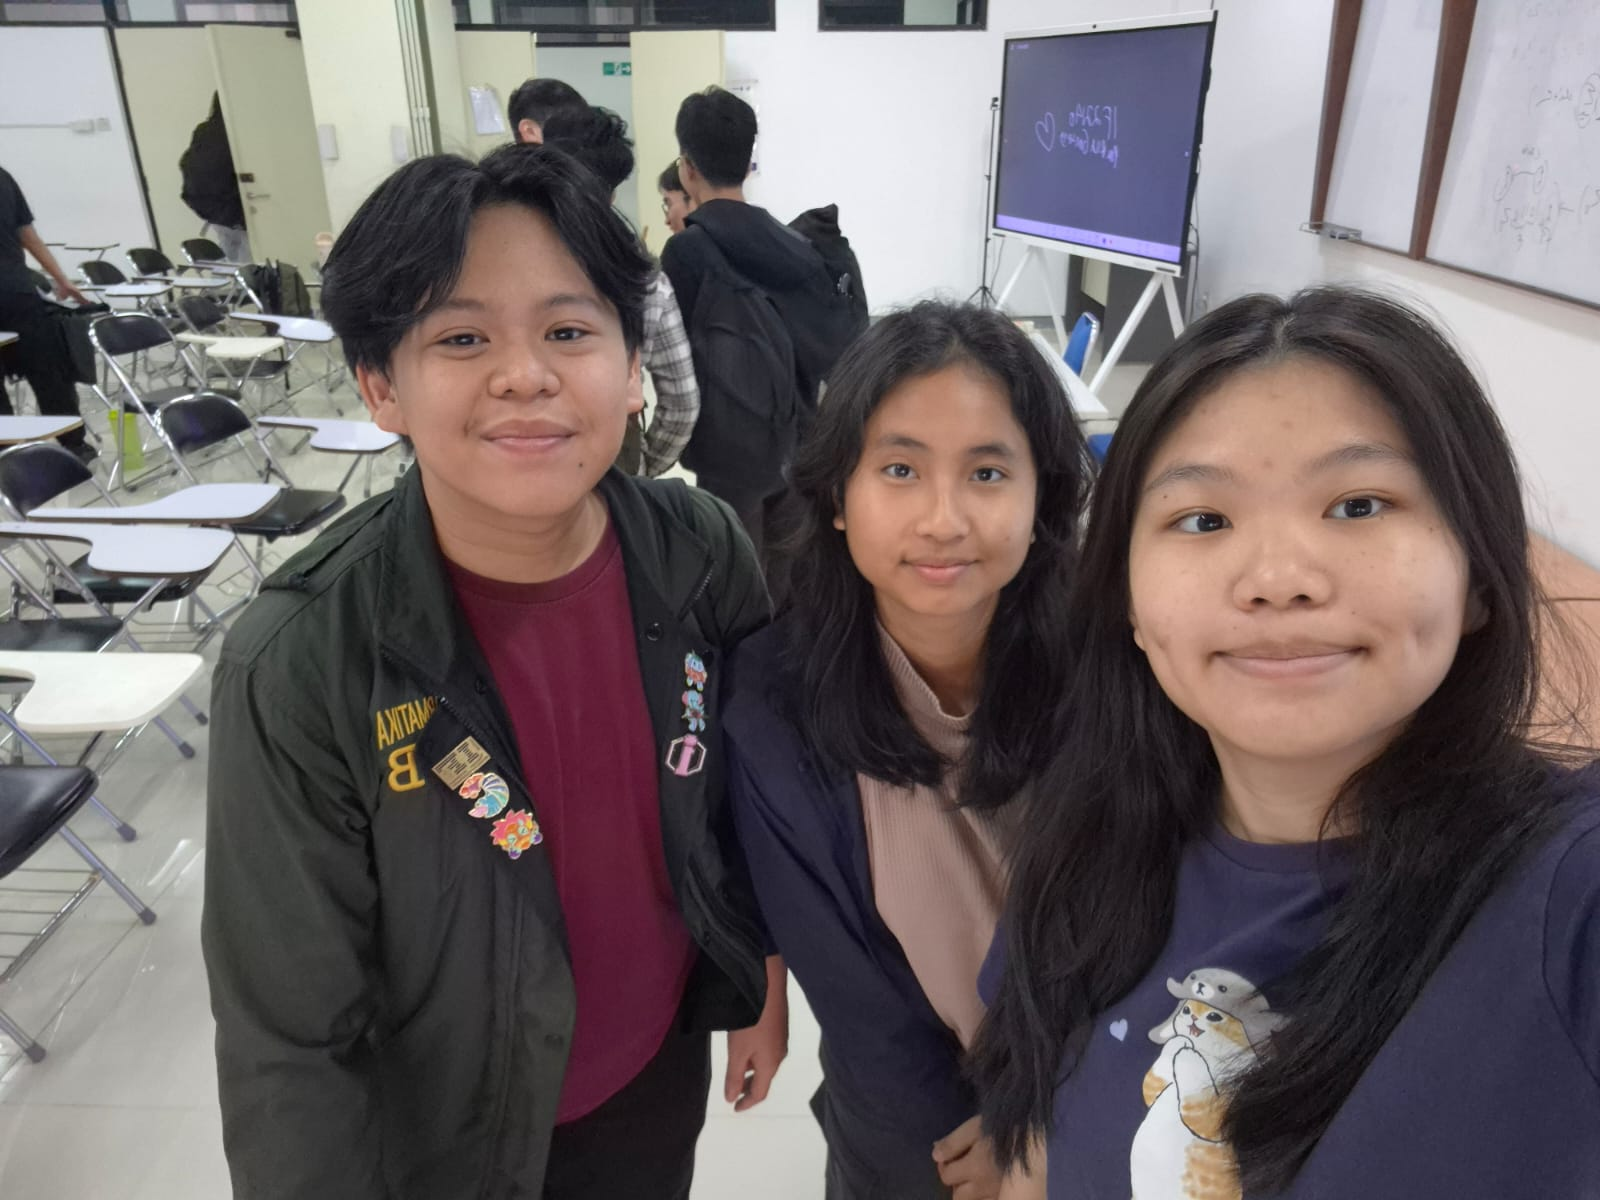
\includegraphics[width=1.3\textwidth,height=0.35\textheight,keepaspectratio]{foto-kelompok.jpeg}\par
		
		% ---------- Disusun oleh ----------
		\vspace{0.6cm}
		{\bfseries Disusun oleh:\par}
		\vspace{0.2cm}
		\textbf{Berry-Manuka}
		\vspace{0.5cm} \\
		\begin{tabular}{l l}
			Agatha Tatianingseto        & (13524008) \\
			Stefani Angeline Oroh       & (13524064) \\
			Athilla Zaidan Zidna Fann   & (13524068) \\
		\end{tabular}
		
		% ---------- Institusi ----------
		\vspace{1.5cm}
		Laboratorium Ilmu dan Rekayasa Komputasi\par
		Program Studi Teknik Informatika\par
		Sekolah Teknik Elektro dan Informatika\par
		Institut Teknologi Bandung\par
		
	\end{titlepage}
	
	\clearpage
	\pagestyle{fancy}
	
	\tableofcontents
	\clearpage
	
	\chapter{Pendahuluan}
	\section{Kisah}

Setiap kali seseorang membuka sebuah halaman web di peramban (\textit{browser}),
terjadi serangkaian proses yang kompleks di balik layar. Peramban mengunduh
dokumen \textit{HyperText Markup Language} (HTML) dari peladen web, kemudian
mengurai dokumen tersebut menjadi sebuah struktur pohon yang disebut
\textit{Document Object Model} (DOM). Struktur pohon inilah yang menjadi
fondasi bagi seluruh proses selanjutnya --- mulai dari penerapan gaya
(\textit{styling}) melalui \textit{Cascading Style Sheets} (CSS), manipulasi
konten secara dinamis melalui JavaScript, hingga proses \textit{rendering}
visual di layar pengguna.

Salah satu mekanisme fundamental dalam pemrosesan halaman web adalah
\textbf{pencocokan CSS Selector}. Ketika seorang pengembang web menuliskan
aturan CSS seperti \texttt{div > p.highlight}, peramban harus menelusuri
seluruh pohon DOM untuk menemukan elemen-elemen yang memenuhi kriteria
tersebut. Proses penelusuran ini pada dasarnya adalah sebuah \textit{tree
traversal} --- mengunjungi node-node dalam pohon secara sistematis hingga
seluruh elemen yang cocok ditemukan.

Dua algoritma traversal yang paling fundamental adalah \textit{Breadth-First
Search} (BFS) dan \textit{Depth-First Search} (DFS). Kedua algoritma ini
memiliki strategi penelusuran yang berbeda: BFS menjelajahi pohon
secara melebar (\textit{level-by-level}), sementara DFS menjelajahi pohon
secara mendalam (\textit{sedalam mungkin baru mundur}). Pemilihan algoritma
traversal yang tepat dapat memengaruhi efisiensi dan urutan penemuan elemen
yang sesuai dengan CSS Selector yang diberikan.

Pada Tugas Besar 2 mata kuliah IF2211 Strategi Algoritma ini, mahasiswa
diminta untuk membangun sebuah aplikasi web yang mengimplementasikan proses
penelusuran CSS Selector pada pohon DOM menggunakan algoritma BFS dan DFS.
Program yang dikembangkan diberi nama \textbf{Berry-Manuka}: aplikasi web
interaktif yang mampu mengambil dokumen HTML dari suatu URL, mem-parse-nya
menjadi pohon DOM, menelusuri pohon tersebut menggunakan BFS maupun DFS untuk
mencari elemen yang cocok dengan CSS Selector tertentu, serta memvisualisasikan
seluruh proses penelusuran secara interaktif.

\section{Latar Belakang}

\textit{Document Object Model} (DOM) adalah antarmuka pemrograman yang
merepresentasikan struktur dokumen HTML dalam bentuk pohon hierarkis.
Setiap elemen HTML dalam dokumen direpresentasikan sebagai sebuah \textit{node}
dalam pohon, dengan hubungan \textit{parent-child-sibling} yang mencerminkan
struktur bersarang (\textit{nesting}) dari tag-tag HTML \cite{mdn_dom}.
Representasi pohon ini bersifat universal dan menjadi dasar bagi hampir semua
operasi yang dilakukan peramban terhadap halaman web.

Pencocokan CSS Selector merupakan operasi yang sangat sering dilakukan oleh
peramban. Setiap kali sebuah halaman web dimuat, peramban harus mencocokkan
setiap aturan CSS dalam \textit{stylesheet} dengan elemen-elemen yang sesuai
di pohon DOM. Proses ini memerlukan penelusuran pohon DOM secara efisien,
mengingat kompleksitas halaman web modern yang dapat memiliki ribuan hingga
puluhan ribu node \cite{mdn_css_selectors}.

Algoritma \textit{Breadth-First Search} (BFS) dan \textit{Depth-First Search}
(DFS) merupakan dua strategi penelusuran graf dan pohon yang paling dasar dan
penting dalam ilmu komputer \cite{cormen2009introduction}. Kedua algoritma ini
memiliki karakteristik yang berbeda dalam hal urutan kunjungan node, penggunaan
memori, dan kesesuaian dengan jenis pencarian tertentu. Pemahaman mendalam
mengenai perbedaan keduanya sangat penting dalam konteks penelusuran pohon DOM.

Visualisasi interaktif dari proses penelusuran pohon DOM dapat membantu
pengguna memahami cara kerja algoritma BFS dan DFS secara lebih intuitif.
Daripada hanya membaca pseudocode atau analisis teoritis, pengguna dapat
mengamati secara langsung bagaimana setiap algoritma mengunjungi node-node
dalam pohon, mengetahui node mana yang diperiksa terlebih dahulu, dan melihat
jalur yang ditempuh hingga elemen yang dicari ditemukan.

Untuk meningkatkan performa penelusuran pada pohon DOM yang berukuran besar,
diterapkan mekanisme konkurensi menggunakan \textit{goroutine} yang disediakan
oleh bahasa pemrograman Go. Dengan pemrosesan paralel, beberapa node dapat
diperiksa secara bersamaan sehingga waktu penelusuran dapat dikurangi secara
signifikan.

Selain itu, diimplementasikan pula algoritma \textit{Lowest Common Ancestor}
(LCA) dengan metode \textit{Binary Lifting} untuk menentukan ancestor bersama
terdekat dari dua buah node dalam pohon DOM. Algoritma ini memiliki
kompleksitas query sebesar $O(\log N)$, jauh lebih efisien dibandingkan
pendekatan naif yang memiliki kompleksitas $O(N)$ per query
\cite{cpalgorithms_lca}.

\section{Deskripsi Tugas}

Program Berry-Manuka merupakan aplikasi web yang menerima masukan berupa
dokumen HTML --- baik melalui \textit{URL scraping} maupun input manual ---
kemudian mem-parse dokumen tersebut menjadi pohon DOM dan menyediakan
fasilitas penelusuran pohon menggunakan algoritma BFS atau DFS berdasarkan
CSS Selector yang diberikan pengguna. Hasil penelusuran divisualisasikan
secara interaktif lengkap dengan animasi proses penelusuran, statistik
performa, dan traversal log.

Program dikembangkan menggunakan bahasa pemrograman Go untuk \textit{backend}
dan framework Next.js untuk \textit{frontend}, serta dikemas dalam
kontainer Docker untuk memudahkan proses deployment. Program ini dikerjakan
secara berkelompok oleh tiga orang mahasiswa.

\subsection{Masukan}

Program menerima beberapa parameter masukan melalui antarmuka web:

\begin{enumerate}
    \item \textbf{Sumber dokumen HTML}: dapat berupa URL website yang akan
    di-\textit{scrape} atau teks HTML yang dimasukkan secara manual oleh
    pengguna.

    \item \textbf{Pilihan algoritma traversal}: pilihan antara
    \textit{Breadth-First Search} (BFS) atau \textit{Depth-First Search}
    (DFS) sebagai metode penelusuran pohon DOM.

    \item \textbf{CSS Selector}: selector yang digunakan untuk mencari elemen
    yang sesuai dalam pohon DOM. Selector yang didukung meliputi
    \textit{tag selector} (misalnya \texttt{p}), \textit{class selector}
    (misalnya \texttt{.highlight}), \textit{ID selector} (misalnya
    \texttt{\#header}), dan \textit{universal selector} (\texttt{*}), serta
    \textit{combinator} berupa child (\texttt{>}), descendant (spasi),
    adjacent sibling (\texttt{+}), dan general sibling (\texttt{\textasciitilde}).

    \item \textbf{Jumlah hasil}: banyaknya kemunculan elemen yang ingin
    ditampilkan, baik berupa $N$ hasil pertama (\textit{top-N}) maupun
    seluruh kemunculan.
\end{enumerate}

\subsection{Keluaran}

Program menghasilkan beberapa bentuk keluaran melalui antarmuka web:

\begin{enumerate}
    \item \textbf{Visualisasi pohon DOM}: representasi visual dari struktur
    pohon DOM hasil \textit{parsing}, lengkap dengan keterangan kedalaman
    maksimum (\textit{maximum depth}) dari pohon tersebut.

    \item \textbf{Highlight jalur traversal}: penandaan visual pada
    node-node yang dikunjungi selama proses penelusuran, sehingga pengguna
    dapat mengamati urutan dan jalur yang ditempuh oleh algoritma.

    \item \textbf{Animasi penelusuran}: animasi langkah demi langkah dari
    proses penelusuran pohon DOM yang menunjukkan node mana yang sedang
    diperiksa pada setiap tahapan.

    \item \textbf{Statistik performa}: informasi mengenai waktu pencarian
    (dalam milidetik) dan banyaknya node yang dikunjungi selama proses
    penelusuran.

    \item \textbf{Traversal log}: catatan berurutan yang memuat informasi
    setiap tahapan penelusuran, termasuk node yang dikunjungi dan status
    pencocokan terhadap CSS Selector.

    \item \textbf{Lowest Common Ancestor}: hasil pencarian ancestor bersama
    terdekat dari dua buah node yang dipilih oleh pengguna dalam pohon DOM,
    beserta jalur dari masing-masing node menuju ancestor tersebut.
\end{enumerate}

	
	\chapter{Dasar Teori}
	Bagian ini membahas konsep-konsep teoritis yang menjadi landasan pengembangan
program Berry-Manuka. Pemahaman terhadap konsep-konsep berikut diperlukan untuk
memahami cara kerja aplikasi penelusuran pohon DOM menggunakan algoritma
\textit{Breadth-First Search} (BFS) dan \textit{Depth-First Search} (DFS) yang
diimplementasikan.

\section{Document Object Model (DOM)}

\textit{Document Object Model} (DOM) adalah antarmuka pemrograman yang
merepresentasikan struktur dokumen HTML dalam bentuk pohon hierarkis
\cite{mdn_dom}. DOM menyediakan representasi terstruktur dari dokumen, memungkinkan
manipulasi konten, struktur, dan gaya dokumen melalui bahasa pemrograman seperti
JavaScript.

Dalam representasi pohon DOM, setiap elemen HTML dalam dokumen direpresentasikan
sebagai sebuah \textit{node} dalam pohon. Terdapat beberapa tipe node yang
penting:

\begin{itemize}
    \item \textbf{Element node}: merepresentasikan tag HTML seperti \texttt{<div>},
    \texttt{<p>}, atau \texttt{<h1>}. Setiap element node dapat memiliki atribut
    dan children.
    
    \item \textbf{Text node}: merepresentasikan teks yang terdapat di dalam elemen
    HTML. Text node selalu menjadi \textit{leaf node} dalam pohon DOM.
    
    \item \textbf{Attribute node}: merepresentasikan atribut dari sebuah elemen
    HTML seperti \texttt{class}, \texttt{id}, atau \texttt{href}.
\end{itemize}

Struktur pohon DOM memiliki hubungan hierarkis yang mencerminkan struktur
bersarang dari tag-tag HTML:

\begin{itemize}
    \item \textbf{Root node}: \textit{node} paling atas dalam hierarki, biasanya
    elemen \texttt{<html>}, yang merepresentasikan keseluruhan dokumen.
    
    \item \textbf{Parent-child relationship}: setiap node (kecuali root) memiliki
    tepat satu \textit{parent node}, dan setiap node dapat memiliki nol atau
    lebih \textit{child nodes}. Jika node A secara langsung mengandung node B di
    dalamnya, maka A adalah parent dari B dan B adalah child dari A.
    
    \item \textbf{Sibling relationship}: node-node yang memiliki parent yang sama
    disebut \textit{siblings}. Siblings memiliki \textit{previous sibling} dan
    \textit{next sibling} yang menunjukkan urutan kemunculan mereka dalam dokumen.
\end{itemize}

Setiap node dalam pohon DOM memiliki kedalaman (\textit{depth}) yang menunjukkan
jarak dari root node. Root node berada pada kedalaman 0, children langsungnya
pada kedalaman 1, dan seterusnya. Kedalaman maksimum (\textit{maximum depth})
dari pohon menunjukkan tinggi pohon tersebut.

Representasi pohon DOM bersifat universal dan menjadi dasar bagi hampir semua
operasi yang dilakukan peramban terhadap halaman web, termasuk penerapan gaya
CSS, manipulasi konten dinamis, dan pemrosesan event \cite{flanagan2006javascript}.

\section{HTML dan HTML Parsing}

\textit{HyperText Markup Language} (HTML) adalah bahasa markup standar yang
digunakan untuk membuat dan menyusun struktur halaman web \cite{mdn_html}.
HTML menggunakan sistem \textit{tag} untuk menandai berbagai elemen dalam
dokumen seperti teks, gambar, tautan, dan elemen lainnya.

\subsection{Struktur Dasar HTML}

Tag HTML ditulis dengan menggunakan kurung siku sudut (\texttt{< >}). Sebagian
besar tag memiliki tag pembuka (misalnya \texttt{<p>}) dan tag penutup
(misalnya \texttt{</p>}) yang mengapit konten di dalamnya. Terdapat juga tag
yang bersifat \textit{self-closing} atau \textit{void elements} yang tidak
memerlukan tag penutup, seperti \texttt{<br/>}, \texttt{<img/>}, \texttt{<input/>},
\texttt{<hr/>}, \texttt{<meta/>}, dan \texttt{<link/>}.

Setiap elemen HTML dapat memiliki atribut yang memberikan informasi tambahan
atau mengubah perilaku elemen tersebut. Atribut ditulis di dalam tag pembuka
dengan format \texttt{nama="nilai"}. Atribut umum yang sering digunakan antara
lain:

\begin{itemize}
    \item \texttt{class}: menentukan satu atau lebih kelas CSS untuk elemen
    \item \texttt{id}: memberikan identifier unik untuk elemen dalam dokumen
    \item \texttt{href}: menentukan URL tujuan untuk elemen tautan (\texttt{<a>})
    \item \texttt{src}: menentukan sumber file untuk elemen media (\texttt{<img>},
    \texttt{<script>})
\end{itemize}

\subsection{HTML Parsing}

\textit{HTML Parsing} adalah proses membaca dokumen HTML dan mengubahnya menjadi
struktur pohon DOM \cite{whatwg_html}. Parser memproses dokumen secara berurutan
dari awal hingga akhir, mengenali tag-tag HTML dan menyusun hierarki node-node
DOM.

Proses parsing HTML melibatkan beberapa langkah utama:

\begin{enumerate}
    \item \textbf{Tokenization}: membaca karakter demi karakter dari dokumen
    HTML dan mengubahnya menjadi \textit{token} seperti \textit{start tag},
    \textit{end tag}, \textit{attribute}, dan \textit{text}.
    
    \item \textbf{Tree Construction}: membangun pohon DOM berdasarkan token-token
    yang dihasilkan. Proses ini menggunakan \textit{stack} untuk melacak node-node
    yang sedang aktif:
    \begin{itemize}
        \item Saat menemukan \textit{StartTagToken}, sebuah node baru dibuat,
        ditambahkan sebagai child dari node di atas stack, kemudian node baru
        tersebut di-\textit{push} ke stack.
        \item Saat menemukan \textit{EndTagToken}, stack di-\textit{pop} untuk
        kembali ke parent node.
        \item Saat menemukan \textit{SelfClosingTagToken}, node dibuat dan
        ditambahkan sebagai child, tetapi tidak di-\textit{push} ke stack.
        \item \textit{TextToken} ditambahkan sebagai \textit{innerText} dari
        node yang sedang berada di atas stack.
    \end{itemize}
\end{enumerate}

Dalam implementasi program Berry-Manuka, parsing HTML dilakukan menggunakan
pustaka \texttt{golang.org/x/net/html} yang menyediakan \textit{tokenizer} HTML
standar untuk bahasa pemrograman Go. Pustaka ini mampu menangani berbagai kasus
edge seperti tag yang tidak tertutup dengan benar, tag yang bersarang secara
tidak valid, dan karakter khusus dalam dokumen HTML.

\section{CSS Selector}

\textit{Cascading Style Sheets} (CSS) Selector adalah pola yang digunakan untuk
memilih elemen-elemen tertentu dalam pohon DOM agar dapat diberi aturan gaya
\cite{mdn_css_selectors}. Selector memungkinkan pengembang web untuk menargetkan
satu atau lebih elemen berdasarkan tipe tag, atribut class, atribut id, atau
hubungan struktural dengan elemen lain.

\subsection{Selector Dasar}

Program Berry-Manuka mendukung empat tipe selector dasar:

\begin{itemize}
    \item \textbf{Tag Selector}: memilih semua elemen dengan nama tag tertentu.
    Sintaks: \texttt{tagname}. Contoh: \texttt{p} memilih semua elemen \texttt{<p>}.
    
    \item \textbf{Class Selector}: memilih elemen yang memiliki atribut \texttt{class}
    dengan nilai tertentu. Sintaks: \texttt{.classname}. Contoh: \texttt{.box}
    memilih elemen dengan \texttt{class="box"}.
    
    \item \textbf{ID Selector}: memilih elemen yang memiliki atribut \texttt{id}
    dengan nilai tertentu. ID bersifat unik dalam satu dokumen. Sintaks:
    \texttt{\#idname}. Contoh: \texttt{\#header} memilih elemen dengan
    \texttt{id="header"}.
    
    \item \textbf{Universal Selector}: memilih semua elemen dalam dokumen.
    Sintaks: \texttt{*}.
\end{itemize}

\subsection{Combinator}

\textit{Combinator} adalah karakter khusus yang digunakan untuk mengekspresikan
hubungan antara dua selector, memungkinkan pemilihan elemen berdasarkan posisi
relatif mereka dalam pohon DOM. Terdapat empat tipe combinator:

\begin{itemize}
    \item \textbf{Child Combinator} (\texttt{>}): memilih elemen yang merupakan
    \textit{direct child} dari elemen induk tertentu. Contoh: \texttt{div > p}
    memilih elemen \texttt{<p>} yang secara langsung berada di dalam \texttt{<div>}.
    
    \item \textbf{Descendant Combinator} (spasi): memilih elemen yang merupakan
    keturunan (bukan harus direct child) dari elemen tertentu. Contoh:
    \texttt{div p} memilih semua \texttt{<p>} yang berada di dalam \texttt{<div>}
    pada level kedalaman berapa pun.
    
    \item \textbf{Adjacent Sibling Combinator} (\texttt{+}): memilih elemen
    yang merupakan sibling langsung (tepat setelah) elemen tertentu. Contoh:
    \texttt{div + p} memilih \texttt{<p>} yang tepat berada setelah \texttt{<div>}.
    
    \item \textbf{General Sibling Combinator} (\texttt{\textasciitilde}): memilih
    elemen yang merupakan sibling yang berada setelah elemen tertentu (tidak harus
    langsung). Contoh: \texttt{div \textasciitilde p} memilih semua \texttt{<p>}
    yang berada setelah \texttt{<div>} dalam parent yang sama.
\end{itemize}

\subsection{Selector Chain dan Matching}

Selector yang kompleks dapat dibentuk dengan menggabungkan beberapa selector
dan combinator dalam sebuah \textit{chain}. Contoh: \texttt{div > .box p}
berarti memilih elemen \texttt{<p>} yang merupakan descendant dari elemen dengan
class \texttt{box}, yang merupakan direct child dari \texttt{<div>}.

Proses \textit{matching} selector dilakukan dengan memeriksa apakah sebuah node
DOM memenuhi pola selector yang diberikan. Untuk selector chain, matching
dilakukan dari kanan ke kiri, memeriksa hubungan struktural antar elemen sesuai
dengan combinator yang digunakan. Setiap combinator memerlukan pengecekan
hubungan yang berbeda: child combinator memeriksa parent langsung, descendant
combinator menelusuri semua ancestor, dan sibling combinators memeriksa hubungan
sibling dalam parent yang sama.

\section{Breadth-First Search (BFS)}

\textit{Breadth-First Search} (BFS) adalah algoritma traversal graf dan pohon
yang menelusuri node-node secara \textit{level-by-level}, mengunjungi semua node
pada kedalaman tertentu sebelum berpindah ke kedalaman berikutnya
\cite{cormen2009introduction}. Dalam konteks pohon DOM, BFS mengunjungi root
terlebih dahulu, kemudian semua children dari root, kemudian grandchildren, dan
seterusnya.

\subsection{Karakteristik BFS}

BFS menggunakan struktur data \textit{queue} (FIFO --- First In First Out) untuk
mengelola urutan kunjungan node. Root node dimasukkan ke dalam queue terlebih
dahulu. Selama queue tidak kosong, node di depan queue dikeluarkan untuk
diproses, kemudian semua children dari node tersebut dimasukkan ke dalam queue.
Proses ini berulang hingga seluruh node dikunjungi atau target ditemukan.

\subsection{Pseudocode BFS}

Algoritma BFS untuk traversal pohon DOM dengan pencarian berdasarkan CSS selector
dapat dilihat pada Algoritma \ref{alg:bfs}.

\begin{algorithm}
\caption{BFS untuk Penelusuran Pohon DOM}
\label{alg:bfs}
\begin{algorithmic}[1]
\Function{BFS}{$root, selectorChain, limit$}
    \State $queue \gets$ Queue dengan elemen $root$
    \State $visited \gets 0$
    \State $results \gets$ list kosong
    \State $log \gets$ list kosong
    \State $start \gets$ waktu sekarang
    
    \While{$queue$ tidak kosong}
        \State $node \gets queue.$\Call{Dequeue}{}
        \State $visited \gets visited + 1$
        
        \If{\Call{MatchChain}{$node, selectorChain$}}
            \State \Call{Append}{$log, (visited, node, \text{"match"})$}
            \State \Call{Append}{$results, node$}
            \If{$limit > 0$ dan $|results| \geq limit$}
                \State \textbf{break}
            \EndIf
        \Else
            \State \Call{Append}{$log, (visited, node, \text{"visit"})$}
        \EndIf
        
        \For{setiap $child$ dalam $node.Children$}
            \State $queue.$\Call{Enqueue}{$child$}
        \EndFor
    \EndWhile
    
    \State $elapsed \gets$ waktu sejak $start$
    \State \Return \{$results, log, visited, elapsed, \text{"bfs"}$\}
\EndFunction
\end{algorithmic}
\end{algorithm}

\subsection{Analisis Kompleksitas}

Kompleksitas waktu BFS adalah $O(N)$, di mana $N$ adalah jumlah total node dalam
pohon, karena setiap node dikunjungi tepat satu kali. Kompleksitas ruang adalah
$O(W)$, di mana $W$ adalah lebar maksimum pohon (jumlah maksimum node pada satu
level), karena pada saat tertentu queue harus menyimpan semua node pada level
yang sedang diproses.

BFS memiliki karakteristik menemukan elemen pada level atas pohon terlebih dahulu.
Ini menguntungkan ketika elemen target kemungkinan besar berada di level yang
dangkal. Namun, BFS cenderung boros memori pada pohon yang lebar karena harus
menyimpan banyak node dalam queue secara bersamaan.

\section{Depth-First Search (DFS)}

\textit{Depth-First Search} (DFS) adalah algoritma traversal graf dan pohon yang
menelusuri node-node secara mendalam, mengunjungi sejauh mungkin sepanjang setiap
cabang sebelum melakukan \textit{backtrack} \cite{cormen2009introduction}. Dalam
konteks pohon DOM, DFS menelusuri satu subtree secara lengkap sebelum berpindah
ke subtree berikutnya.

\subsection{Karakteristik DFS}

DFS dapat diimplementasikan secara iteratif menggunakan \textit{stack} (LIFO ---
Last In First Out) atau secara rekursif. Dalam implementasi iteratif, root node
dimasukkan ke dalam stack terlebih dahulu. Selama stack tidak kosong, node di
atas stack dikeluarkan untuk diproses, kemudian children dari node tersebut
dimasukkan ke dalam stack dalam urutan terbalik sehingga children paling kiri
 diproses terlebih dahulu.

\subsection{Pseudocode DFS}

Algoritma DFS untuk traversal pohon DOM dengan pencarian berdasarkan CSS selector
dapat dilihat pada Algoritma \ref{alg:dfs}.

\begin{algorithm}
\caption{DFS untuk Penelusuran Pohon DOM}
\label{alg:dfs}
\begin{algorithmic}[1]
\Function{DFS}{$root, selectorChain, limit$}
    \State $stack \gets$ Stack dengan elemen $root$
    \State $visited \gets 0$
    \State $results \gets$ list kosong
    \State $log \gets$ list kosong
    \State $start \gets$ waktu sekarang
    
    \While{$stack$ tidak kosong}
        \State $node \gets stack.$\Call{Pop}{}
        \State $visited \gets visited + 1$
        
        \If{\Call{MatchChain}{$node, selectorChain$}}
            \State \Call{Append}{$log, (visited, node, \text{"match"})$}
            \State \Call{Append}{$results, node$}
            \If{$limit > 0$ dan $|results| \geq limit$}
                \State \textbf{break}
            \EndIf
        \Else
            \State \Call{Append}{$log, (visited, node, \text{"visit"})$}
        \EndIf
        
        \For{$i \gets |node.Children| - 1$ downto $0$}
            \State $stack.$\Call{Push}{$node.Children[i]$}
        \EndFor
    \EndWhile
    
    \State $elapsed \gets$ waktu sejak $start$
    \State \Return \{$results, log, visited, elapsed, \text{"dfs"}$\}
\EndFunction
\end{algorithmic}
\end{algorithm}

\subsection{Analisis Kompleksitas}

Kompleksitas waktu DFS adalah $O(N)$, di mana $N$ adalah jumlah total node dalam
pohon, sama seperti BFS. Namun, kompleksitas ruang DFS adalah $O(H)$, di mana $H$
adalah tinggi maksimum pohon (kedalaman terdalam dari leaf node), karena stack
hanya menyimpan node-node pada satu path dari root ke leaf yang sedang dijelajahi.

DFS lebih hemat memori pada pohon yang lebar karena tidak perlu menyimpan semua
node pada satu level. DFS juga menemukan elemen pada kedalaman tertentu lebih
cepat daripada BFS. Namun, DFS tidak menjamin menemukan elemen pada level yang
dangkal terlebih dahulu, yang dapat menjadi kelemahan jika target kemungkinan
besar berada di level atas pohon.

\section{Perbandingan BFS dan DFS}

BFS dan DFS merupakan dua algoritma traversal fundamental yang memiliki
karakteristik berbeda dalam hal urutan kunjungan node, penggunaan memori, dan
kesesuaian dengan berbagai skenario pencarian. Tabel \ref{tab:bfs-dfs-comparison}
menyajikan perbandingan komprehensif antara kedua algoritma.

\begin{table}[H]
\centering
\caption{Perbandingan Algoritma BFS dan DFS}
\label{tab:bfs-dfs-comparison}
\begin{tabular}{|p{4cm}|p{5cm}|p{5cm}|}
\hline
\textbf{Aspek} & \textbf{BFS} & \textbf{DFS} \\
\hline
Struktur Data & Queue (FIFO) & Stack (LIFO) \\
\hline
Urutan Kunjungan & Level-by-level & Depth-first (subtree lengkap dulu) \\
\hline
Kompleksitas Waktu & $O(N)$ & $O(N)$ \\
\hline
Kompleksitas Ruang & $O(W)$ --- lebar maksimum pohon & $O(H)$ --- tinggi maksimum pohon \\
\hline
Menemukan Top-Level Duluan & Ya & Tidak \\
\hline
Menemukan Deep Element Duluan & Tidak & Ya \\
\hline
Cocok untuk Pohon Lebar & Boros memori & Hemat memori \\
\hline
Cocok untuk Pohon Dalam & Hemat memori & Boros memori (jika sangat dalam) \\
\hline
\end{tabular}
\end{table}

\subsection{Pemilihan Algoritma yang Tepat}

Pemilihan antara BFS dan DFS bergantung pada karakteristik pohon DOM dan sifat
pencarian yang dilakukan:

\begin{itemize}
    \item \textbf{Gunakan BFS} ketika:
    \begin{itemize}
        \item Elemen target kemungkinan besar berada di level dangkal pohon
        \item Pohon memiliki struktur yang dalam (tidak terlalu lebar)
        \item Perlu menemukan elemen terdekat dari root
        \item Memori tidak menjadi kendala utama
    \end{itemize}
    
    \item \textbf{Gunakan DFS} ketika:
    \begin{itemize}
        \item Elemen target kemungkinan besar berada di kedalaman tertentu
        \item Pohon memiliki struktur yang lebar (banyak children per node)
        \item Perlu menelusuri satu subtree lengkap sebelum berpindah
        \item Penggunaan memori perlu diminimalkan
    \end{itemize}
\end{itemize}

Dalam konteks penelusuran CSS Selector pada pohon DOM, kedua algoritma dapat
digunakan bergantung pada pola dokumen HTML yang umum dijumpai. BFS menguntungkan
untuk selector yang menargetkan elemen umum seperti \texttt{<p>} atau \texttt{<div>}
yang biasanya tersebar di berbagai level. DFS menguntungkan untuk selector dengan
combinator descendant (\texttt{div p}) karena dapat menelusuri satu cabang pohon
secara lengkap.

\section{Web Scraping}

\textit{Web scraping} adalah teknik ekstraksi data dari situs web dengan
mengambil konten halaman web dan mengubahnya menjadi format yang dapat diproses
secara terstruktur \cite{w3school_scraping}. Dalam konteks program Berry-Manuka,
web scraping digunakan untuk mengambil dokumen HTML dari URL yang diberikan
pengguna sebelum dokumen tersebut diparse menjadi pohon DOM.

\subsection{HTTP Client dan Request Handling}

Proses web scraping dimulai dengan membuat HTTP request ke URL target menggunakan
\textit{HTTP client}. Request yang umum digunakan untuk mengambil halaman web adalah
HTTP GET request. HTTP client mengirimkan request ke peladen web dan menerima
response yang berisi status code, headers, dan body (konten halaman).

Headers dalam HTTP response memberikan informasi penting seperti:
\begin{itemize}
    \item \texttt{Content-Type}: menunjukkan tipe konten (harus \texttt{text/html}
    untuk dokumen HTML)
    \item \texttt{Content-Length}: ukuran konten dalam bytes
    \item \texttt{Status Code}: hasil permintaan (200 OK untuk sukses)
\end{itemize}

\subsection{Validasi dan Error Handling}

Beberapa aspek penting dalam implementasi web scraping yang robust:

\begin{itemize}
    \item \textbf{URL Validation}: memastikan URL valid dengan skema yang benar
    (\texttt{http://} atau \texttt{https://}) dan format yang sesuai.
    
    \item \textbf{Timeout}: membatasi waktu tunggu response untuk mencegah program
    hang jika peladen tidak merespons. Timeout yang umum digunakan adalah 10-30
detik.
    
    \item \textbf{Size Limit}: membatasi ukuran konten yang diunduh untuk mencegah
    penggunaan memori yang berlebihan. Batas yang umum adalah 5-10 MB.
    
    \item \textbf{Error Handling}: menangani berbagai skenario error seperti
    connection timeout, DNS resolution failure, HTTP error codes (404, 500, dll),
    dan invalid content type.
\end{itemize}

\subsection{Security Considerations}

Web scraping perlu memperhatikan aspek keamanan dan etika:

\begin{itemize}
    \item \textbf{Robots.txt}: menghormati file \texttt{robots.txt} yang menentukan
    bagian situs mana yang boleh atau tidak boleh di-scrape.
    \item \textbf{Rate Limiting}: tidak membuat request terlalu sering ke satu
    situs untuk menghindari beban berlebih pada peladen.
    \item \textbf{Static vs Dynamic Content}: web scraping menggunakan HTTP client
    standar hanya dapat mengambil konten \textit{static}. Konten yang dirender
    menggunakan JavaScript (\textit{dynamic content}) memerlukan tools khusus
    seperti \textit{headless browser}.
\end{itemize}

Dalam implementasi Berry-Manuka, web scraping dilakukan menggunakan paket
\texttt{net/http} dari bahasa Go yang menyediakan HTTP client dengan dukungan
\textit{timeout}, \textit{redirect handling}, dan validasi \textit{content-type}.

\section{Lowest Common Ancestor dan Binary Lifting}

\textit{Lowest Common Ancestor} (LCA) dari dua node dalam pohon adalah node
terdalam yang merupakan ancestor dari kedua node tersebut \cite{cpalgorithms_lca}.
Dalam konteks pohon DOM, LCA merepresentasikan elemen kontainer terdekat yang
mengandung kedua elemen yang dipilih.

\subsection{Definisi LCA}

Diberikan pohon $T$ dengan root $r$ dan dua node $u$ dan $v$ dalam pohon tersebut,
LCA dari $u$ dan $v$ (dinotasikan $\text{LCA}(u, v)$) adalah node $w$ dengan
kedalaman maksimum sedemikian sehingga $w$ adalah ancestor dari $u$ dan $w$
juga adalah ancestor dari $v$.

\subsection{Pendekatan Naive}

Pendekatan sederhana untuk mencari LCA adalah dengan menelusuri parent dari
kedua node secara bersamaan hingga ditemukan node yang sama. Algoritma ini:
\begin{enumerate}
    \item Samakan kedalaman kedua node dengan menggerakkan node yang lebih dalam
    ke atas (menuju parent) hingga kedalaman sama.
    \item Gerakkan kedua node ke atas bersamaan hingga keduanya bertemu di node
    yang sama. Node pertemuan tersebut adalah LCA.
\end{enumerate}
Kompleksitas pendekatan naive adalah $O(N)$ per query dalam kasus terburuk,
di mana $N$ adalah jumlah node dalam pohon.

\subsection{Binary Lifting}

\textit{Binary Lifting} adalah teknik optimasi yang memungkinkan query LCA dalam
kompleksitas $O(\log N)$ dengan preprocessing $O(N \log N)$ \cite{bender2000lca}.
Teknik ini menggunakan tabel \textit{sparse table} untuk menyimpan ancestor
$2^k$ dari setiap node.

\subsubsection{Preprocessing}

Didefinisikan $\text{up}[v][k]$ sebagai ancestor ke-$2^k$ dari node $v$:
\begin{itemize}
    \item $\text{up}[v][0] = \text{parent}(v)$ (ancestor $2^0 = 1$)
    \item $\text{up}[v][k] = \text{up}[\text{up}[v][k-1]][k-1]$ untuk $k > 0$
    (ancestor $2^k$ adalah ancestor $2^{k-1}$ dari ancestor $2^{k-1}$)
\end{itemize}

Tabel diisi menggunakan BFS atau DFS dari root. Nilai $\text{MAXLOG}$ dipilih
sedemikian sehingga $2^{\text{MAXLOG}} > N$. Untuk pohon dengan hingga sekitar
1 juta node, $\text{MAXLOG} = 20$ sudah mencukupi karena $2^{20} = 1.048.576$.

\subsubsection{Query LCA}

Algoritma query LCA dengan Binary Lifting:
\begin{enumerate}
    \item \textbf{Samakan kedalaman}: jika $\text{depth}[u] > \text{depth}[v]$,
    tukar $u$ dan $v$. Kemudian naikkan $u$ menggunakan binary lifting hingga
    $\text{depth}[u] = \text{depth}[v]$.
    
    \item \textbf{Binary lift bersama}: jika $u = v$ setelah langkah 1, return $u$.
    Jika tidak, naikkan $u$ dan $v$ bersamaan dari $k = \text{MAXLOG}-1$ hingga
    $0$, tetapi hanya jika $\text{up}[u][k] \neq \text{up}[v][k]$. Ini memastikan
    kita tidak melewati LCA.
    
    \item \textbf{Return parent}: LCA adalah parent dari $u$ (atau $v$), yaitu
    $\text{up}[u][0]$.
\end{enumerate}

Teknik ini juga memungkinkan rekonstruksi jalur dari suatu node ke root dengan
kompleksitas $O(\log N)$ per node dalam jalur.

\section{Konkurensi dan Goroutine}

\textit{Concurrency} adalah kemampuan suatu program untuk menjalankan beberapa
tugas secara bersamaan atau tumpang tindih dalam waktu \cite{donovan2015go}.
Concurrency berbeda dengan \textit{parallelism}: concurrency berkaitan dengan
struktur program yang memungkinkan beberapa tugas berjalan secara bersamaan,
sedangkan parallelism berkaitan dengan eksekusi fisik beberapa tugas secara
simultan pada beberapa prosesor.

\subsection{Goroutine}

\textit{Goroutine} adalah unit eksekusi ringan (\textit{lightweight}) yang
disediakan oleh bahasa pemrograman Go untuk mendukung concurrency. Berbeda dengan
\textit{thread} pada umumnya yang dikelola oleh sistem operasi, goroutine
dikelola oleh \textit{runtime} Go sehingga lebih efisien dalam penggunaan memori
(biasanya hanya beberapa KB) dan lebih cepat dalam pembuatan serta penghancurannya.

Goroutine dibuat dengan menambahkan kata kunci \texttt{go} sebelum pemanggilan
fungsi:
\begin{verbatim}
go namaFungsi(argumen)
\end{verbatim}

Program utama (\texttt{main}) dan semua goroutine yang aktif berjalan secara
concurrent, memungkinkan pemanfaatan multi-core processor untuk parallelism.

\subsection{Sinkronisasi dengan WaitGroup}

\textit{WaitGroup} dari paket \texttt{sync} adalah mekanisme sinkronisasi yang
memungkinkan sebuah goroutine menunggu selesainya sejumlah goroutine lain.
WaitGroup memiliki tiga metode utama:
\begin{itemize}
    \item \texttt{Add(n)}: menambah counter sebesar $n$
    \item \texttt{Done()}: mengurangi counter (dipanggil oleh goroutine yang
    selesai)
    \item \texttt{Wait()}: blok sampai counter mencapai nol
\end{itemize}

\subsection{Thread Safety dengan Mutex}

\textit{Mutex} (\textit{mutual exclusion}) dari paket \texttt{sync} adalah
mekanisme penguncian yang memastikan hanya satu goroutine yang mengakses
sumber daya bersama pada satu waktu. Ini mencegah \textit{race condition}
ketika beberapa goroutine mengakses dan memodifikasi data bersama secara
bersamaan.

Mutex memiliki dua metode utama:
\begin{itemize}
    \item \texttt{Lock()}: mengakuisisi lock. Jika lock sedang dipegang goroutine
    lain, goroutine ini akan blok sampai lock tersedia.
    \item \texttt{Unlock()}: melepaskan lock, memungkinkan goroutine lain
    mengakuisisinya.
\end{itemize}

\subsection{Parallel BFS dan DFS}

\textit{Parallel BFS} dapat diimplementasikan dengan memproses semua node pada
level yang sama secara paralel menggunakan goroutine. Setiap node diproses
oleh goroutine terpisah, dan hasilnya dikumpulkan menggunakan mutex untuk
melindungi akses ke struktur data bersama.

\textit{Parallel DFS} dapat diimplementasikan dengan memproses setiap subtree
langsung dari root secara paralel. Setiap child dari root diproses oleh
goroutine terpisah yang menjalankan DFS sequential pada subtree tersebut.

Keuntungan parallel traversal tergantung pada ukuran pohon dan struktur hardware.
Untuk pohon yang cukup besar, overhead pembuatan goroutine dapat diimbangi oleh
gain dari eksekusi paralel. Namun, untuk pohon kecil, sequential traversal
mungkin lebih cepat karena tidak ada overhead sinkronisasi.

\section{Containerization dan Docker}

\textit{Containerization} adalah teknik virtualisasi tingkat sistem operasi yang
memungkinkan aplikasi dan dependensinya dikemas dalam sebuah \textit{container}
yang terisolasi \cite{docker_docs}. Container menyediakan lingkungan runtime
yang konsisten dan portable, memastikan aplikasi berjalan sama di berbagai
environment (development, testing, production).

\subsection{Konsep Container}

Container berbeda dengan \textit{virtual machine} (VM) tradisional. VM
mengemulasikan seluruh sistem operasi termasuk kernel, sedangkan container
berbagi kernel sistem operasi host dan hanya mengisolasi proses, filesystem,
dan network namespace. Ini membuat container jauh lebih ringan dan cepat
dibandingkan VM.

Keuntungan menggunakan container:
\begin{itemize}
    \item \textbf{Portability}: aplikasi dalam container dapat berjalan di
    environment mana pun yang mendukung container runtime
    \item \textbf{Isolation}: setiap container memiliki filesystem, proses, dan
    network yang terpisah, mencegah konflik antar aplikasi
    \item \textbf{Efficiency}: container menggunakan sumber daya lebih efisien
daripada VM karena berbagi kernel OS
    \item \textbf{Scalability}: container dapat dengan mudah direplikasi dan
di-\textit{orchestrate} menggunakan tools seperti Docker Compose atau Kubernetes
\end{itemize}

\subsection{Docker}

Docker adalah platform containerization yang paling populer, menyediakan tools
untuk membangun, menjalankan, dan mengelola container. Komponen utama Docker
meliputi:

\begin{itemize}
    \item \textbf{Docker Engine}: runtime container yang menjalankan container
    \item \textbf{Dockerfile}: file konfigurasi yang mendefinisikan cara membangun
    \textit{image} container
    \item \textbf{Docker Image}: template read-only untuk membuat container
    \item \textbf{Docker Compose}: tool untuk mendefinisikan dan menjalankan
    multi-container applications
\end{itemize}

\subsection{Dockerfile dan Multi-Stage Builds}

\textit{Dockerfile} mendefinisikan instruksi untuk membangun image container.
\textit{Multi-stage builds} adalah teknik yang menggunakan beberapa \texttt{FROM}
statements dalam satu Dockerfile, memungkinkan pemisahan antara environment
build dan runtime.

Keuntungan multi-stage builds:
\begin{itemize}
    \item Mengurangi ukuran final image dengan hanya menyertakan artifacts yang
    diperlukan (binary executable), tidak termasuk tools build
    \item Meningkatkan keamanan dengan tidak menyertakan compiler atau tools
    development dalam image production
    \item Mempercepat deployment karena image yang lebih kecil lebih cepat di-push
    dan di-pull
\end{itemize}

\subsection{Docker Compose}

\textit{Docker Compose} adalah tool untuk mendefinisikan dan menjalankan
aplikasi multi-container. Dengan menggunakan file \texttt{docker-compose.yml},
seluruh stack aplikasi (frontend, backend, database, dll) dapat didefinisikan
secara deklaratif dan dijalankan dengan satu perintah.

Docker Compose mengelola:
\begin{itemize}
    \item Pembuatan dan konfigurasi container
    \item Network antara container
    \item Volume untuk persistent storage
    \item Dependency dan urutan startup antar services
    \item Environment variables dan port mapping
\end{itemize}

Dalam konteks program Berry-Manuka, Docker Compose digunakan untuk mengorkestrasi
dua container: backend (Go) dan frontend (Next.js), memastikan kedua service
dapat berkomunikasi dan dijalankan bersama dengan konfigurasi yang konsisten.

	
	\chapter{Aplikasi BFS dan DFS}
	\input{sections/03-implementasi}
	
	\chapter{Implementasi}
	\section{Gambaran Umum Sistem}

Aplikasi yang dikembangkan merupakan sistem berbasis web yang bertujuan untuk melakukan pencarian elemen HTML pada struktur DOM berdasarkan CSS selector. Sistem ini memanfaatkan algoritma Breadth First Search (BFS) dan Depth First Search (DFS) sebagai metode traversal.

\begin{tcolorbox}[colback=gray!10,title=Input dan Output Sistem]
\textbf{Input:}
\begin{itemize}
    \item URL website atau teks HTML
    \item CSS Selector
    \item Pilihan algoritma (BFS / DFS)
    \item Jumlah hasil
\end{itemize}

\textbf{Output:}
\begin{itemize}
    \item Elemen hasil pencarian
    \item Visualisasi DOM
    \item Jalur traversal
    \item Waktu eksekusi
\end{itemize}
\end{tcolorbox}

% --------ARSITEKTUR SISTEM--------

\section{Arsitektur Sistem}

Sistem dibangun dengan pendekatan client-server.

\begin{center}
\begin{tabular}{|c|c|c|}
\hline
Frontend & $\rightarrow$ & Backend \\
\hline
Input user & & Parsing + BFS/DFS \\
\hline
Visualisasi & $\leftarrow$ & Hasil traversal \\
\hline
\end{tabular}
\end{center}

\begin{itemize}
    \item Frontend: menerima input dan menampilkan hasil
    \item Backend: melakukan parsing HTML dan traversal DOM
\end{itemize}

	
	\chapter{Penutup}
	\section{Kesimpulan}
 
Berdasarkan hasil implementasi dan pengujian yang telah dilakukan, dapat ditarik beberapa kesimpulan sebagai berikut.
 
\begin{enumerate}
    \item Aplikasi traversal pohon DOM berbasis web berhasil dibangun menggunakan React/Next.js pada \textit{frontend} dan Go pada \textit{backend}, dengan arsitektur \textit{client-server} melalui REST API. Aplikasi berhasil di-\textit{deploy} secara publik menggunakan Microsoft Azure Virtual Machine dan dapat diakses melalui \texttt{http://40.81.27.55:3000}.
 
    \item Proses \textit{scraping} HTML dari URL eksternal dan \textit{parsing} HTML menjadi struktur pohon DOM berjalan dengan benar. Parser mampu menangani berbagai jenis elemen HTML termasuk elemen \textit{void}, atribut, dan konten teks, serta menolak input yang tidak valid dengan pesan \textit{error} yang sesuai.
 
    \item Implementasi CSS \textit{selector} berhasil mendukung empat jenis \textit{selector} dasar (\textit{tag}, \textit{class}, \textit{ID}, \textit{universal}) serta empat jenis kombinator (\textit{child}, \textit{descendant}, \textit{adjacent sibling}, \textit{general sibling}) dengan mekanisme pencocokan dari kanan ke kiri yang mengikuti standar CSS.
 
    \item Algoritma BFS dan DFS berhasil diimplementasikan dengan benar. BFS menelusuri pohon DOM secara \textit{level-by-level} sehingga cenderung menemukan elemen yang lebih dangkal terlebih dahulu, sedangkan DFS menelusuri secara \textit{pre-order} sehingga menyelami satu cabang hingga tuntas sebelum berpindah ke cabang berikutnya. Perbedaan perilaku keduanya terlihat jelas terutama saat parameter \textit{Top N} digunakan, di mana urutan penemuan node pertama dapat berbeda secara signifikan.
 
    \item Parameter \textit{Top N} terbukti tidak sekadar memfilter tampilan hasil, melainkan secara nyata menghentikan proses traversal lebih awal sehingga mengurangi jumlah node yang dikunjungi dan mempersingkat \textit{traversal log}.
 
    \item Parallel BFS berhasil memparalelkan pemrosesan seluruh node dalam satu level menggunakan \textit{goroutine}, menghasilkan kumpulan node yang identik dengan BFS sekuensial. Parallel DFS memparalelkan pemrosesan subtree di level pertama di bawah root, menghasilkan urutan traversal yang identik dengan DFS sekuensial setelah di-\textit{sort} berdasarkan indeks.
 
    \item Algoritma LCA dengan teknik \textit{Binary Lifting} berhasil diimplementasikan dan dapat menemukan leluhur bersama terendah dari dua node yang dipilih melalui antarmuka visualisasi pohon DOM. \textit{Preprocessing} tabel \textit{sparse table} dengan \texttt{maxLog} = 20 memungkinkan penanganan pohon dengan kedalaman hingga $2^{20}$ level.
 
    \item Seluruh 47 \textit{test case} yang dirancang berhasil dijalankan sesuai \textit{expected output}.
\end{enumerate}
 
\section{Saran}
 
Berdasarkan hasil implementasi dan temuan selama pengujian, beberapa saran untuk pengembangan lebih lanjut adalah sebagai berikut.
 
\begin{enumerate}
    \item Memperluas cakupan paralelisasi Parallel DFS agar tidak hanya terbatas pada level pertama di bawah root, melainkan dapat memparalelkan pemrosesan secara rekursif pada setiap level subtree sehingga peningkatan performa lebih signifikan pada pohon DOM yang sangat besar.
 
    \item Menambahkan dukungan CSS \textit{selector} yang lebih lengkap seperti \textit{attribute selector} (\texttt{[attr=value]}), \textit{pseudo-class} (\texttt{:first-child}, \texttt{:nth-child}), dan \textit{pseudo-element} untuk meningkatkan kompatibilitas dengan standar CSS yang sesungguhnya.
 
    \item Menambahkan mekanisme \textit{caching} pada hasil \textit{scraping} URL yang sama sehingga permintaan berulang pada URL yang tidak berubah tidak perlu melakukan \textit{fetch} ulang ke server target.
 
    \item Meningkatkan batasan ukuran HTML yang dapat diproses (saat ini 5 MB) serta menambahkan penanganan untuk halaman web yang membutuhkan eksekusi JavaScript (\textit{dynamic rendering}) menggunakan \textit{headless browser}.
 
    \item Menambahkan fitur ekspor pohon DOM ke format gambar atau PDF langsung dari antarmuka web sehingga memudahkan dokumentasi hasil penelusuran.
\end{enumerate}

	\chapter{Lampiran}
	
\section{Tautan Repository GitHub}
 
Repository kode sumber aplikasi dapat diakses pada tautan berikut.
 
\begin{itemize}
    \item \textbf{Repository:} \url{https://github.com/AthillaZaidan/Tubes2_Berry-Manuka}
\end{itemize}
 
%-------

\section{Tabel Pembagian Tugas}
 
\begin{table}[H]
\centering
\caption{Pembagian Tugas Anggota Kelompok}
\label{tab:pembagian-tugas}
\renewcommand{\arraystretch}{1.5}
\begin{tabular}{|c|p{3.5cm}|p{2.5cm}|p{5cm}|}
\hline
\textbf{No} & \textbf{Nama} & \textbf{NIM} & \textbf{Tugas} \\
\hline
1 & Agatha Tatianingseto & 13524008 & Backend dan Laporan \\
\hline
2 & Stefani Angeline Oroh & 13524064 & Frontend dan Laporan \\
\hline
3 & Athilla Zaidan Zidna Fann & 13524068 & Backend dan Laporan \\
\hline
\end{tabular}
\end{table}
 
%-------

\section{Tabel Checklist}
 
\begin{table}[H]
\centering
\caption{Checklist Pemenuhan Spesifikasi}
\label{tab:checklist}
\renewcommand{\arraystretch}{1.5}
\begin{tabular}{|c|p{9cm}|c|c|}
\hline
\textbf{No} & \textbf{Poin} & \textbf{Ya} & \textbf{Tidak} \\
\hline
1 & Aplikasi berhasil dikompilasi tanpa kesalahan & \checkmark & \\
\hline
2 & Aplikasi berhasil dijalankan & \checkmark & \\
\hline
3 & Aplikasi dapat menerima input URL web, pilihan algoritma, CSS \textit{selector}, dan jumlah hasil & \checkmark & \\
\hline
4 & Aplikasi dapat melakukan \textit{scraping} terhadap web pada input & \checkmark & \\
\hline
5 & Aplikasi dapat menampilkan visualisasi pohon DOM & \checkmark & \\
\hline
6 & Aplikasi dapat menelusuri pohon DOM dan menampilkan hasil penelusuran & \checkmark & \\
\hline
7 & Aplikasi dapat menandai jalur tempuh oleh algoritma & \checkmark & \\
\hline
8 & Aplikasi dapat menyimpan jalur yang ditempuh algoritma dalam \textit{traversal log} & \checkmark & \\
\hline
9 & {[Bonus]} Membuat video & & \checkmark \\
\hline
10 & {[Bonus]} \textit{Deploy} aplikasi & \checkmark & \\
\hline
11 & {[Bonus]} Implementasi animasi pada penelusuran pohon & \checkmark & \\
\hline
12 & {[Bonus]} Implementasi \textit{multithreading} & \checkmark & \\
\hline
13 & {[Bonus]} Implementasi LCA \textit{Binary Lifting} & \checkmark & \\
\hline
\end{tabular}
\end{table}

\clearpage
\section{Pernyataan}
\begin{center}
\begin{tabular}{|p{13cm}|}
\hline
\\
Tugas ini disusun sepenuhnya tanpa bantuan kecerdasan buatan (\textit{Generative AI}),
melainkan hasil pemikiran dan analisis mandiri.

\vspace{2cm}

\begin{flushright}
\begin{tabular}{c}

\includegraphics[width=3cm]{ttd1.png} \\
\underline{Agatha Tatianingseto} \\[1.5cm]
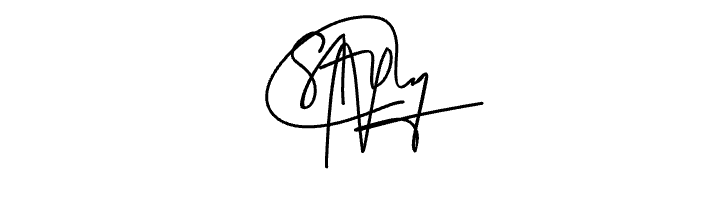
\includegraphics[width=5cm]{ttd2.png} \\
\underline{Stefani Angeline Oroh} \\[1.3cm]

\includegraphics[width=2cm]{ttd3.png} \\
\underline{Athilla Zaidan Zidna Fann} \\[1cm]
\end{tabular}
\end{flushright}

\\
\hline
\end{tabular}
\end{center}

	
	\bibliography{dafpus}
	
\end{document}
